%%%%%%%%%%%%%%%%%%%%%%% file template.tex %%%%%%%%%%%%%%%%%%%%%%%%%
%
% This is a general template file for the LaTeX package SVJour3
% for Springer journals.          Springer Heidelberg 2010/09/16
%
% Copy it to a new file with a new name and use it as the basis
% for your article. Delete % signs as needed.
%
% This template includes a few options for different layouts and
% content for various journals. Please consult a previous issue of
% your journal as needed.
%
%%%%%%%%%%%%%%%%%%%%%%%%%%%%%%%%%%%%%%%%%%%%%%%%%%%%%%%%%%%%%%%%%%%
%
% First comes an example EPS file -- just ignore it and
% proceed on the \documentclass line
% your LaTeX will extract the file if required
\begin{filecontents*}{example.eps}
%!PS-Adobe-3.0 EPSF-3.0
%%BoundingBox: 19 19 221 221
%%CreationDate: Mon Sep 29 1997
%%Creator: programmed by hand (JK)
%%EndComments
gsave
newpath
  20 20 moveto
  20 220 lineto
  220 220 lineto
  220 20 lineto
closepath
2 setlinewidth
gsave
  .4 setgray fill
grestore
stroke
grestore
\end{filecontents*}
%
\RequirePackage{fix-cm}
%
%\documentclass{svjour3}                     % onecolumn (standard format)
%\documentclass[smallcondensed]{svjour3}     % onecolumn (ditto)
%\documentclass[smallextended]{svjour3}       % onecolumn (second format)
\documentclass[twocolumn]{svjour3}          % twocolumn
%
\smartqed  % flush right qed marks, e.g. at end of proof
%
\usepackage{graphicx}
\usepackage[round]{natbib}
\usepackage{amsmath}  
\usepackage{amsfonts} 
\usepackage{graphicx} 
\usepackage[usenames]{color}
\usepackage{mathtools}
\usepackage{algorithm}
\usepackage[noend]{algpseudocode}
\usepackage{float}
%
% \usepackage{mathptmx}      % use Times fonts if available on your TeX system
%
% insert here the call for the packages your document requires
%\usepackage{latexsym}
% etc.
%
% please place your own definitions here and don't use \def but
% \newcommand{}{}
\newcommand{\Real}{\mathbb R}
\newcommand{\E}{\mathbb{E}}
\newcommand{\s}{\mathbb{S}}
\renewcommand{\P}{\mathbb{P}}
\newcommand{\K}{\mathbb{K}}
\newcommand{\Q}{\mathbb{Q}}
\newcommand{\eps}{\varepsilon}
\newcommand{\diag}{\mathrm{diag}}
\newcommand{\nbr}{\mathrm{nbr}}
\newcommand{\F}{\mathcal{F}}
\newcommand{\M}{\mathcal{M}}
\newcommand{\Z}{\mathcal{Z}}
\newcommand{\csimplex}{\bar{\mathcal{S}}^{d-1}}
\newcommand{\osimplex}{\mathcal{S}^{d-1}}
\newcommand{\LL}{\mathcal{L}}
\newcommand{\Hil}{\mathscr{H}}
\newcommand{\G}{\mathscr{G}}
\newcommand{\p}{\mathscr{P}}
\newcommand{\C}{\mathscr{C}}
\newcommand{\one}[1]{\mathbf{1}_{\{#1\}}}
\newcommand{\oneset}[1]{\mathbf{1}_{#1}}
\newcommand{\argmin}{\mathrm{argmin}}
\newcommand{\argmax}{\mathrm{argmax}}
\newcommand{\var}{\mathrm{Var}}
\newcommand{\cov}{\mathrm{Cov}}
\newcommand{\ind}{\mathrm{I}}
\newcommand{\D}{\mathscr{D}}
\newcommand{\Borel}{\mathscr{B}}
\newcommand{\ben}{\begin{enumerate}}
\newcommand{\een}{\end{enumerate}}
\newcommand{\ds}{\displaystyle}
\newcommand{\voila}{\hfill $\blacksquare$}
\newcommand{\Id}{\mathrm{Id}}
\renewcommand{\Re}{\mathrm{Re}}
\renewcommand{\vec}[1]{\mathbf{#1}}
\renewcommand{\d}[1]{\ensuremath{\operatorname{d}\!{#1}}}
%
% Insert the name of "your journal" with
% \journalname{myjournal}
%
\begin{document}
\bibliographystyle{plainnat}

\title{Sequential Importance Sampling With Corrections For Partially Observed States
%\thanks{Grants or other notes
%about the article that should go on the front page should be
%placed here. General acknowledgments should be placed at the end of the article.}
}

%\titlerunning{Short form of title}        % if too long for running head

\author{Valentina Di Marco         \and
        Jonathan Keith \and
        Daniel Spring
}

%\authorrunning{Short form of author list} % if too long for running head

\institute{Valentina Di Marco \at
              School of Mathematical Science, Monash University, Clayton Campus, VIC 3800, Australia \\
              Tel.: +61-4-23330509\\
              \email{valentina.dimarco@monash.edu}           %  \\
%             \emph{Present address:} of F. Author  %  if needed
           \and
           Jonathan Keith \at
              School of Mathematical Science, Monash University, Clayton Campus, VIC 3800, Australia
	   \and
	  Daniel Spring \at
	      School of Ecosystem and Forest Sciences, The University of Melbourne, Parkville, Victoria 3010, Australia
}

\date{Received: date / Accepted: date}
% The correct dates will be entered by the editor


\maketitle

\begin{abstract}

We consider an evolving system for which a sequence of observations is being made, with each observation revealing additional information about current and past states of the system. We suppose each observation is made without error, but does not fully determine the state of the system at the time it is made. Our motivating example is drawn from invasive species biology, where it is common to know the precise location of invasive organisms that have been detected by a surveillance program, but at any time during the program there are invaders that have not been detected.

We propose a sequential importance sampling strategy to infer parameters under a Bayesian model of such a system. The strategy involves simulating multiple alternative states consistent with current knowledge of the system, as revealed by the observations. However, a difficult problem that arises is that observations made at a later time are invariably incompatible with previously simulated states.

To solve this problem, we propose a two-step iterative process in which states of the system are alternately simulated in accordance with past observations, then corrected in light of new observations. We identify criteria under which such corrections can be made while maintaining appropriate importance weights.

\keywords{ Sequential Importance Sampling \and Filtering \and Bayesian estimation \and Partially observed spaces \and Missing data}
% \PACS{PACS code1 \and PACS code2 \and more}
% \subclass{MSC code1 \and MSC code2 \and more}
\end{abstract}

\section{Introduction}
This paper considers the problem of imputing missing data in the presence of incomplete observations made sequentially in real time. We thus envisage data that consists of a series of correlated observations made sequentially in time, each of which is correct but only partially reveals the true state of the system. The main difficulty that arises in this context is that data missing at one time point can be revealed at a later time point, so that imputed missing values must later be corrected in light of new information.

Our original motivation for considering this problem was to facilitate analysis of the Red Imported Fire Ant (RIFA) invasion in Queensland, Australia, where in an ongoing surveillance program, the locations of ants’ nests are regularly being detected. For detected nests, the location can be precisely determined, but at any given time there is an unknown number of undetected nests, each with an unknown location. To infer the current extent of the invasion, we aim to impute plausible locations of undetected individuals, but these imputations are only informed guesses, and will require constant correction as new detections come to light.

In addition, new nests are constantly being produced: the unseen state of the system is thus constantly evolving. Knowing the location of at least some of the invaders at time $t$, we can simulate the evolution of this system. However, again the imputed locations of simulated nests will require constant correction as more information about the true state of the system becomes available.

In this paper, we propose a new approach to problems of this type. Although our approach is ultimately aimed at inference for invasive species, here we will illustrate the method for less complex evolving systems in which correct but partial observations are being made in real time.

To handle problems of this kind, we introduce a Bayesian approach that uses a new sequential importance sampling (SIS) strategy. As is typical of SIS methods, we generate a population of particles, each representing a plausible sequence of system states, and we evolve each particle at each time step according to a model of system dynamics. Again in a manner typical of SIS methods, new observations arrive in real time, and we use these observations to adjust the weights assigned to particles. However, a crucial new element in our method is that we allow missing values imputed at earlier time steps to be corrected so that they are consistent with the new observations.

Our method thus addresses a problem that is common in practice: new observations made in real time can render previously imputed missing values implausible, and may even conflict with what has been simulated. For example, in the invasive species context described above, undetected nests imputed to geographic areas that do not contain any nests become increasingly implausible as time passes without detections being made in those regions. In standard SIS approaches, such particles receive low weights and are eventually eliminated by resampling, but a common problem is that all particles can become implausible, if not inconsistent, with observations.

Problems of this kind arise in many contexts. We can envisage the approach being used to study the evolution of a species' geographic range, for both invasive and non-invasive species. The algorithm could be also applied to a variety of other missing data problems where new incomplete data is continuously acquired, like in crime prediction, (\cite{Malathy}) or bushfire modeling (\cite{Beer}). Another potential application is in the study of the spread of infectious diseases, where observations are made in the form of diagnosed cases, but missing data in the form of undiagnosed cases is unavoidable (\cite{O'Neill}). 

Missing data are ubiquitous in ecological and evolutionary data sets as in any other branch of science. The common methods used to deal with missing data are to delete cases containing missing data, and to use the mean to fill in missing values. However, these ‘traditional’ methods result in biased estimation of parameters and uncertainty, and reduction in statistical power. Better missing data procedures such as data augmentation (\cite{Tanner}) and multiple imputation (\cite{RubinMI}) are readily available and implementable (\cite{Nakagawa}).

Particle filters are used to estimate a hidden state when partial (noisy) observations are made. However, the standard particle filtering algorithm can diverge or its performance can severely degrade in the presence of missing data (\cite{Zhang}).

On the other hand, multiple imputations do not use past observations and the state transition equations when estimating the probability of the hidden state knowing the observations. This can result in poor performance when the problem can be well modelled by a Markov structure (\cite{Zhang}).

In the context of missing observations, \cite{Zhang} have developed a Multiple Imputation Particle Filter (MIPF) to deal with these deficiencies. This method uses randomly drawn values (imputations) to provide a replacement for the missing data and then uses the particle filter to estimate non-linear state with the data.

Data Augmentation methods in Bayesian statistic are normally used to evaluate an intractable posterior distribution of the parameters when data can be augmented in such a way that it become easy to analyse the augmented data (\cite{Tanner}).

In our method we will use data augmentation in sequential importance sampling in order to simulate the new state of the system using a first set of samples and a second sample corrected in light of new data acquired at each step.

Our method deals with situations where the data are informative, a situation where standard sequential Monte Carlo methods can perform poorly. 

Similarly, \cite{Del Moral} have proposed a Sequential Monte Carlo method for sampling the posterior distribution of state-space models under highly informative observation regimes. In their method they introduce a schedule of intermediate weighting and resampling times between observation times, which guide particles towards the final state.

A similar method was used by Finke et al. (2018) who developed a Particle Monte Carlo Markov Chain algorithm to estimate the demographic parameters of a population and then incorporated this algorithm into a sequential Monte Carlo sampler in order to perform model comparison motivated by the fact that a simple importance sampling performs poorly if there is a strong mismatch between the prior and the posterior, which is common when the data is highly informative.

In this paper we provide a proof of concept for our proposed methodology using a simple system modelled by an AR(1) process. In section HHH we present a version of our method in which only those imputed values that are strictly inconsistent with later observations are corrected, in a deterministic manner. In Section HHH we generalise this approach to allow non-deterministic revision of imputed values that, while not inconsistent with later observations, can nevertheless be updated in light of new information.

\section{Sequential Importance Sampling with corrections for the AR1 model}

Let us first introduce our importance sampling idea using a simple example.

Consider a linear, normal and stationary AR(1) process for which

\[
x_{t} = \varphi x_{t-1} + \eps_{t}
\]
with $\eps_{t} \stackrel{iid}{\sim} \mathcal{N}(0, \sigma^{2})$.
Then

\[
(x_{t} | x_{t-1}) \sim \mathcal{N} (\varphi x_{t-1}, \sigma^{2}).
\]
This process is stationary provided that the initial distribution is

\[
x_{1} \sim \mathcal{N} \Bigg (0, \frac{\sigma^2}{1- \varphi^2} \Bigg )
\]
which is valid only if $|\varphi| < 1$.

Suppose that at any time $t$, only some subset of the values $\vec {x}^{(t)} = (x_1, \dots, x_{t})$ have so far been observed. However, those that have been observed are known without error. We collect the values that have been observed at or before time $t$ to form a vector $\vec{z}^{(t)} = (z_1^{(t)}, \dots, z_{t}^{(t)})$, where for each $s \leq t$, $z_s^{(t)} = x_s$ if $x_s$ has been observed at or before time $t$ and $z_s^{(t)} = -$ otherwise. Thus the coordinates of $\vec{z}^{(t)}$ belong to an extension of the reals $\mathbb{R} \cup \{ - \}$.

As time progresses, new observations become available. Thus some dashes in the vector $\vec{z}^{(t)}$ will be replaced by observations in the subsequent vector $\vec{z}^{(t+1)}$. However, the reverse does not occur: if we have $z_s^{(t)} = x_s$ for times $s$ and $t$ where $s \leq t$ then we must also have $z_s^{(t^{\prime})} = x_s$ at all subsequent times $t^{\prime} > t$.

We will therefore define a lower triangular $t \times t$ matrix $\vec{Z}^{(t)}$ in which row $i$ is the vector $\vec{z}^{(i)}$.

We will also define binary vectors $\vec{b}^{(t)} = (b_1^{(t)}, \dots, b_{t}^{(t)})$, where $b_s^{(t)} = 1$ if $z_s^{(t)} = x_s$, and $b_s^{(t)} = 0$ if $z_s^{(t)} = -$, and a lower triangular $t \times t$ binary matrix $\vec{B}^{(t)}$ in which row $i$ is the vector $\vec{b}^{(i)}$.
The matrix $\vec{B}^{(t)}$ must satisfy the constraints that if $B_{ij}^{(t)} = b_j^{(i)} = 1$ for $i \in \{ 1, \ldots, t \}$ and $j \in \{ 1, \ldots, i \}$, then $B_{mj}^{(t)} = 1$ for all $m \in \{ i+1, \ldots, t \}$.

Note $\vec{b}^{(t)}$ is fully determined by $\vec{z}^{(t)}$.

We will model $b_j^{(i)}$, when $b_j^{(i-1)} = 0$ as Bernoulli with probability $\theta$:
\[
(b_j^{(i)} | b_j^{(i-1)} = 0) \sim Bernoulli(\theta).
\]




\subsection{Bayesian inference in a partially observed state space}

To perform Bayesian inference in this partially observed state space we want to determine the posterior distribution for the pairs $(\vec{x}^{(t)}, \vec{B}^{(t)})$ in light of observations $\vec{Z}^{(t)}$. Suppose that at time $t$ we have some prior density $q(\vec{x}^{(t)},\vec{B}^{(t)} | \vec{Z}^{(t-1)})$ that represents our knowledge about the state before we observe $\vec{z}^{(t)}$. This prior is defined on the subspace $\Omega = \Omega_1 \times \Omega_2$ where $\Omega_1 = \prod_{s=1}^t \mathbb{X}_s^{(t-1)} \subseteq \mathbb{R}^t$ and $\Omega_2 = \prod_{s=1}^t \mathbb{B}_s^{(t-1) \times (t-1)} \subseteq 2^{(t \times t)}$ is such that $\mathbb{X}_s^{(t-1)} = \mathbb{R}$ for $b_s^{(t-1)} = 0$ or $s=t$, and $\mathbb{X}_s^{(t-1)} = \{ x_s \}$ for $b_s^{(t-1)} = 1$. Also, $\vec{b}^{(t)}$ evolves independently of $\vec{x}^{(t)}$, so that the distribution of $\vec{b}^{(t)}$ is a conditional probability of the form $P(\vec{b}^{(t)} | \vec{x}^{(t)}, \vec{z}^{(t-1)} ) = P( \vec{b}^{(t)} | \vec{b}^{(t-1)} )$. Under these conditions, the posterior distribution for the pair $(\vec{x}^{(t)}, \vec{B}^{(t)})$ is obtained by re-normalising $q$ over values consistent with $\vec{Z}^{(t)}$. In other words, it has a density on the subspace $\Omega' = \Omega'_1 \times \Omega'_2$ where $\Omega'_1 = \prod_{s=1}^t \mathbb{X}_s^{(t)} \subseteq \mathbb{R}^t$ and and $\Omega'_2 = \prod_{s=1}^t \mathbb{B}_s^{(t \times t)} \subseteq 2^{(t \times t)}$ such that $\mathbb{X}_s^{(t)} = \mathbb{R}$ for $b_s^{(t)} = 0$ and $\mathbb{X}_s^{(t)} = \{ z_s^{(t)}\}$ for $b_s^{(t)} = 1$, given by:
\[
p(\vec{x}^{(t)}, \vec{B}^{(t)} | \vec{Z}^{(t)})  =   
\frac{ q(\vec{x}^{(t)}, \vec{B}^{(t)}|\vec{Z}^{(t-1)})} {r(\vec{Z}^{(t)} | \vec{Z}^{(t-1)})}
\]
where 
\[
r(\vec{Z}^{(t)} | \vec{Z}^{(t-1)}) = \int q(\vec{x}^{(t)}, \vec{B}^{(t)}|\vec{Z}^{(t-1)}) \prod_{\{s \leq t: b_s^{(t)} = 0\}} dx_s^{(t)}.
\]

This follows from Bayes' Rule, but we omit the proof to keep the example simple. A proof for a more general context is provided below (HHH TO DO).

The prior for time $t$, $q(\vec{x}^{(t)},\vec{B}^{(t)} | \vec{Z}^{(t-1)})$ represents our knowledge about the state before we observe $\vec{z}^{(t)}$. In our toy example, using the independence of the processes $x$ and $B$, we have
\begin{multline}
    q(\vec{x}^{(t)},\vec{B}^{(t)} | \vec{Z}^{(t-1)}) = \\ q(\vec{x}^{(t-1)},\vec{B}^{(t-1)} | \vec{Z}^{(t-1)}) p(x_t | x_{t-1}) p(\vec{b}^{(t)} | \vec{b}^{(t-1)}).
\end{multline}


\subsection{Sequential importance sampling with an auxiliary variable in a partially observed state space}

We want to approximate the distribution 

\[
p(\vec{x}^{(t)}, \vec{B}^{(t)} | \vec{Z}^{(t)})
\]
iteratively, as well as related properties including

\[
    p(x_{t}, \vec{b}^{(t)} | \vec{Z}^{(t)})
\]
and expectations of the form:
\begin{multline*}
E_{p} \Big[f(\vec{x}^{(t)}, \vec{B}^{(t)}) \Big] = \\
\int f(\vec{x}^{(t)}, \vec{B}^{(t)})\; p(\vec{x}^{(t)}, \vec{B}^{(t)} | \vec{Z}^{(t)})\; d\vec{x}^{(t)}
\end{multline*}
for functions $f: \Omega  \rightarrow \Real$. 

We take a sequential importance sampling approach, at each iteration using a collection of weighted particles to represent $p(\vec{x}^{(t-1)}, \vec{B}^{(t-1)} | \vec{Z}^{(t-1)})$ from the previous iteration, in the sense that these particles can be used to construct weighted Monte Carlo estimates for integrals of the above form. We evolve these under the model to create a new set of weighted particles representing the prior for iteration $t$, namely $q(\vec{x}^{(t)}, \vec{B}^{(t)} | \vec{Z}^{(t-1)})$. We then modify these particles to be consistent with the observations $\vec{Z}^{(t)}$, and adjust the weights to ensure the resulting weighted particles represent $p(\vec{x}^{(t)}, \vec{B}^{(t)} | \vec{Z}^{(t)})$.

Consider a particle $(\vec{x}^{(t-1)},\vec{B}^{(t-1)})$ constructed at time point $t$, one of $n$ such particles. We generate a new value $x_t$ for this particle by drawing $p(x_t | x_{t-1})$. Similarly, we generate a new value $\vec{b}^{(t)}$ for this particle by drawing from $p(\vec{b}^{(t)} | \vec{b}^{(t-1)})$ (see equation $(1)$). However, the new vector of observations $\vec{z}^{(t)}$ is typically inconsistent with a particle $(\vec{x}^{(t)}, \vec{B}^{(t)})$ thus constructed, in two ways: first, the coordinates at which $\vec{b}^{(t)}$ contains a 0 may not correspond to the coordinates at which $\vec{z}^{(t)}$ contains a `-', and second, the observed values in $\vec{z}^{(t)}$ differ from the corresponding coordinates of $\vec{x}^{(t)}$. We must therefore correct $\vec{x}^{(t)}$ and $\vec{b}^{(t)}$ in light of the new observations $\vec{z}^{(t)}$. The simplest way to do this is to first replace $\vec{b}^{(t)}$ with the unique binary vector $\vec{b'}^{(t)}$ that is consistent with $\vec{z}^{(t)}$, and then replace the coordinates of $\vec{x}^{(t)}$ with the corresponding coordinates of $\vec{z}^{(t)}$ wherever $\vec{b'}^{(t)}$ has a `1', thus generating a corrected term $\vec{x'}^{(t)}$. The corrections thus made at time point $t$ will be carried forward into the particles used at all future times. Note that in this simple example the corrections are deterministic, that is, $\vec{x'}^{(t)}$ and $\vec{b'}^{(t)}$ are deterministic functions of $\vec{x}^{(t)}$ and $\vec{b}^{(t)}$. 

At each iteration, in order to simulate via a two-step process in which we generate a sample and then correct in light of data, we propose to introduce an auxiliary variable into importance sampling. The auxiliary variable will be the yet to be corrected sample $(\vec{x}^{(t)}, \vec{B}^{(t)})$ at time $t$. We will use a projection map $\pi$ to relate the augmented space $\Omega_{\vec{Z}^{(t)}}$ containing the elements $(\vec{x'}^{(t)}, \vec{B'}^{(t)}, \vec{x}^{(t)}, \vec{B}^{(t)})$ to the corrected state space $\Omega'$ containing $(\vec{x'}^{(t)}, \vec{B'}^{(t)})$. Then, we apply importance sampling to be able to estimate the posterior distribution $p(\vec{x}^{(t)}, \vec{B}^{(t)} | \vec{Z}^{(t)})$ or the expectation

\[
E_{p}[f(\vec{x}^{(t)},\vec{B}^{(t)})]
\]
sampling from the known distribution $q$.

For simplicity, let us call $(\vec{x}^{(t)}, \vec{B}^{(t)}) = \vec{y}^{(t)}$ and $(\vec{x'}^{(t)}, \vec{B'}^{(t)}) = \vec{y'}^{(t)}$

Our strategy is to define a probability $p^*$ on $\Omega_{\vec{z}^{(t)}}$ such that the marginal distribution of $p^*$ on $\Omega'$ is $p$, that is:

\[
p(\vec{y'}^{(t)} | \vec{Z}^{(t)}) = \int p^*(\vec{y'}^{(t)}, \vec{y}^{(t)} | \vec{Z}^{(t)})\; d\vec{y}^{(t)}
\]
By the the disintegration theorem it follows that:

\begin{multline*}
E_{p}[f(\vec{y'}^{(t)})]  = \int_{\Omega'} f(\vec{y'}^{(t)})\; p(\vec{y'}^{(t)} | \vec{Z}^{(t)}) d \vec{y'}^{(t)} \\
= \int_{\Omega'} f(\vec{y'}^{(t)})\Bigg[\int_{\pi^{-1}} p^*(\vec{y'}^{(t)}, \vec{y}^{(t)} | \vec{Z}^{(t)}) d\vec{y}^{(t)}\Bigg] d\vec{y'}^{(t)} \\ 
= \int_{\Omega_{\vec{Z}^{(t)}}} f(\pi(\vec{y'}^{(t)}, \vec{y}^{(t)}))\; p^*(\vec{y'}^{(t)}, \vec{y}^{(t)} | \vec{Z}^{(t)}) d \vec{y}^{(t)} \\ 
= E_{p^*}[f(\pi (\vec{y'}^{(t)}, \vec{y}^{(t)}))].
\end{multline*}
Using importance sampling

\begin{multline*}
E_{p^*}[f(\pi (\vec{y'}^{(t)}, \vec{y}^{(t)})] = \int_{\Omega_{\vec{Z}^{(t)}}} f(\pi(\vec{y'}^{(t)},  \vec{y}^{(t)})) \\ \frac{p^*(\vec{y'}^{(t)}, \vec{y}^{(t)}|\vec{Z}^{(t)})} {q(\vec{y'}^{(t)}, \vec{y}^{(t)} | \vec{Z}^{(t-1)})} q(\vec{y'}^{(t)}, \vec{y}^{(t)} | \vec{Z}^{(t-1)}) \; d\vec{y}^{(t)} \\ 
\approx \sum_{j=1}^n  w^{(t)_j}f(\pi (\vec{y'}^{(t)_j}, \vec{y}^{(t)_j}))
\end{multline*}
Where the weights $w^{(t)_j}$ are:

\[
w^{(t)_j} = \frac{p^*(\vec{y'}^{(t)_j}, \vec{y}^{(t)_j} | \vec{Z}^{(t)})} {q(\vec{y'}^{(t)_j}, \vec{y}^{(t)_j}|\vec{Z}^{(t-1)})}
\]
In our example with deterministic substitutions $p^*$ will simply be:

\[
p^*(\vec{y'}^{(t)}, \vec{y}^{(t)} | \vec{Z}^{(t)}) = p(\vec{y'}^{(t)} | \vec{Z}^{(t)}) = \frac{ q(\vec{y'}^{(t)}|\vec{Z}^{(t-1)})} {r(\vec{Z}^{(t)} | \vec{Z}^{(t-1)})}
\]
and

\[
q(\vec{y'}^{(t)}, \vec{y}^{(t)} | \vec{Z}^{(t-1)}) = q(\vec{y}^{(t)} | \vec{Z}^{(t-1)})
\]
therefore the normalised weights $w_t$ will be:

\begin{multline*}
w^{(t)_j} = \frac{q(\vec{y'}^{(t)_j} | \vec{Z}^{(t-1)}) }{q(\vec{y}^{(t)_j} | \vec{Z}^{(t-1)})}\Bigg( \sum_{j=1}^n  \frac{q(\vec{y'}^{(t)_j} | \vec{Z}^{(t-1)}) }{q(\vec{y}^{(t)_j} | \vec{Z}^{(t-1)})}\Bigg)^{-1} = \\
\frac{q(\vec{x'}^{(t)_j}, \vec{B'}^{(t)_j} | \vec{Z}^{(t-1)}) }{q(\vec{x}^{(t)_j}, \vec{B}^{(t)_j} | \vec{Z}^{(t-1)})}\Bigg( \sum_{j=1}^n \frac{q(\vec{x'}^{(t)_j}, \vec{B'}^{(t)_j} | \vec{Z}^{(t-1)}) }{q(\vec{x}^{(t)_j}, \vec{B}^{(t)_j} | \vec{Z}^{(t-1)})}\Bigg)^{-1}
\end{multline*}
since the constant $r$ of $q(\vec{x}^{(t-1)_j},\vec{B}^{(t-1)_j} | \vec{Z}^{(t-1)})$ cancels out after normalisation.

Notice that since we are correcting every previous event at every iteration, the weights for the previous times too will need to be recalculated at every iteration. However, we will now show that there will be many cancellations in the calculation of the weights, making the process manageable and not computationally expensive.

For every particle $j$, the unnormalised weights at time $t$ for $b' \in \{0,1\}$ and $b \in \{0,1\}$ are calculated with the following formula

\begin{multline*}
w^{(t)} = \frac{q(\vec{y'}^{(t)} | \vec{Z}^{(t-1)}) }{q(\vec{y}^{(t)} | \vec{Z}^{(t-1)})} = \\
\frac{\bigg \{ \prod_{i=2}^{N}  \frac{1}{\sqrt{2 \pi \sigma^{2}}} \exp \bigg [ { - \frac{1}{2 \sigma^{2}} }  (x'_{i} - \varphi x'_{i-1})^{2} \bigg ] \bigg \} }{\bigg \{ \prod_{i=2}^{N}  \frac{1}{\sqrt{2 \pi \sigma^{2}}} \exp \bigg [ { - \frac{1}{2 \sigma^{2}} }  (x_{i} - \varphi x_{i-1})^{2} \bigg ] \bigg \} } \\
\frac{p(x'_{1}) \prod_{i=1}^{N} p^{b'_i} (1 - p)^{1-b'_{i}}  }{ p(x_{1}) \prod_{i=1}^{N} p^{b_i} (1 - p)^{1-b_{i}} }
\end{multline*}
and we will have terms cancellations in the Gaussian term when both $z_{i-1} \neq 0$ and $z_{i} \neq 0$, while the Bernoulli term will cancel every time that $z_{i} \neq 0$. Also, we will consider that the first event is known a priori, so that $p(x'_1)=p(x_1)$, and those two terms will cancel out as well.



\subsection{The pseudo-code for the AR(1) model with deterministic corrections}

\begin{algorithm}[H]
\caption{SIR with deterministic corrections for an AR(1) model}\label{euclid}
 \begin{algorithmic}

 \State  \bf{Initialize:} \normalfont At time i = 1
            
\begin{enumerate}
	\item For $j = 1, \dots , n$
	\begin{enumerate}
		\item Sample $x_{1}^{(j)} \sim \mathcal{N} \Bigg (0, \frac{\sigma^2}{1- \varphi^2} \Bigg)$ and sample $b_1^{(j)} \sim Bernoulli(\theta)$
		\item Evaluate the importance weights up to a normalising constant:
		\[
		\tilde{w}^{(j)}_{1} = 1
		\]
	\end{enumerate}
	\item For $j = 1, \dots , n$ normalise the importance weights: 
	\[
	w^{(j)}_{1} = \frac{1}{n}
	\]
\end{enumerate}

 \State  \bf{Iterate:} \normalfont For $i$ from 2 to $N$

\begin{enumerate}
	\item For $j = 1, \dots , n$
	\begin{enumerate}
  		\item sample $x_{i}^{(j)} \sim \mathcal{N} (\varphi x_{i-1}^{(j)}, \sigma^{2})$ and $\vec{b}_i^{(j)} \sim Bernoulli(\theta)$.
		\item {If we had new observations, correct every element of $\vec{x}_{i}^{(j)}$ in light of the data $\vec{z}_{i}$ to obtain new samples $\vec{x'}_{i}^{(j)}$ directly substituting the new data: for $m = 1, \dots ,i$ if $z_{m} \neq -$, $(x')_m^{(j)} = z_{m}$ else if $z_{m} = -$, $(x')_m^{(j)} = x_m^{(j)}$.}
		\item {Correct every element of $\vec{b}_{i}^{(j)}$ in light of the data $\vec{z}_{i}$ to obtain new samples $\vec{b'}_{i}^{(j)}$ substituting 0s when $z_i = -$ and 1s otherwise.}
		\item Evaluate the importance weights up to a normalising constant:
		\[
		\tilde{w}^{(j)}_{i} = \frac{q(\vec{x'}^{(i)_j}, \vec{B'}^{(i)_j} | \vec{Z}^{(i-1)})}{q(\vec{x}^{(i)_j}, \vec{B}^{(i)_j} | \vec{Z}^{(i-1)})}
		\]
	\end{enumerate}
	\item For $j = 1, \dots , n$ normalise the importance weights:
	\[
	w^{(j)}_{i} = \frac{\tilde{w}^{(j)}_{i}}{\sum_{k=1}^{n}\tilde{w}^{(k)}_{i}}
	\]
	\item Perform resampling
	\begin{enumerate}
	    \item Draw N particles from the current particle set with probabilities proportional to their weights. Replace the current particle set with the new N particles
	    \item For $j=1,\cdots ,n$ set $w_{i}^{(j)}=1/n$
	\end{enumerate}
	

\end{enumerate}

\State  \bf{Output:} \normalfont $\Big \{ x_{i}^{(j)} , w_{i}^{(j)} \Big \}_{j = 1}^{n}$ for $i \in \{ 1, N \}$

\item Calculate the expectation  $E[x_i] = \sum_{k=1}^{n} x^{(k)}_i w_{i}^{(k)}$
  
 \end{algorithmic}
\end{algorithm}

\section{The non-deterministic corrections}

In this section we will add non-deterministic corrections to our algorithm. Specifically, every substitution we make based on observations will have an effect on the simulated adjacent unobserved events: the algorithm will substitute each observed elements and also correct the previous element and the following element if they are unobserved. We will be sampling an unobserved event at times $s\leq t$ where $t$ is the current time, with probability $H(x'_s|x'_{s-1}, x'_{s+1})$.

The probability $H(x'_s|x'_{s-1}, x'_{s+1})$ will have the form:

\begin{multline*}
H(x'_s|x'_{s-1}, x'_{s+1}) = \\
\begin{cases} p(x'_s|x'_{s-1}), & \mbox{if} \quad b'_s = 0 \quad b'_{s-1} = 1 \quad b'_{s+1} = 0 \\ 
p(x'_s|x'_{s+1}) & \mbox{if} \quad b'_s = 0 \quad b_{s-1} = 0 \quad b'_{s+1} = 1\\
\frac{p(x'_s|x'_{s-1})p(x'_{s+1}|x'_s)}{p(x'_s)} & \mbox{if} \quad b'_s = 0 \quad b'_{s-1} = 1 \quad b'_{s+1} = 1\\
1 & \mbox{otherwise} \end{cases}
\end{multline*}
We already know that $p(x'_s|x'_{s-1}) \sim \mathcal{N} (\varphi x_{s}, \sigma^{2})$. Also, for a stationary AR(1) model, the marginal distribution for every value of $s$ is $p(x_{s}) \sim \mathcal{N}(0, v)$ where $v = Var(x_s)$ is the variance of $x_s$. Since the process is stationary, (linear and Gaussian), it is also time reversible and using Bayes theorem it can be shown that 
\[
p(x'_{s}|x'_{s+1}) \sim \mathcal{N} (\varphi x'_{s+1}, \sigma^{2})
\]
as well.

This new terms will be introduced in the calculation of the weights

%\section{Section title}
%\label{sec:1}
%Text
%\subsection{Subsection title}
%\label{sec:2}
%as required. Don't forget to give each section
%and subsection a unique label (see Sect.~\ref{sec:1}).
%\paragraph{Paragraph headings} Use paragraph headings as needed.
%\begin{equation}
%a^2+b^2=c^2
%\end{equation}

% For one-column wide figures use
%\begin{figure}
% Use the relevant command to insert your figure file.
% For example, with the graphicx package use
%  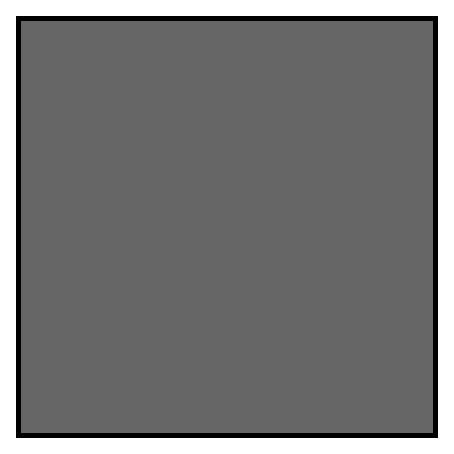
\includegraphics{example.eps}
% figure caption is below the figure
%\caption{Please write your figure caption here}
%\label{fig:1}       % Give a unique label
%\end{figure}
%
% For two-column wide figures use
%\begin{figure*}
% Use the relevant command to insert your figure file.
% For example, with the graphicx package use
%  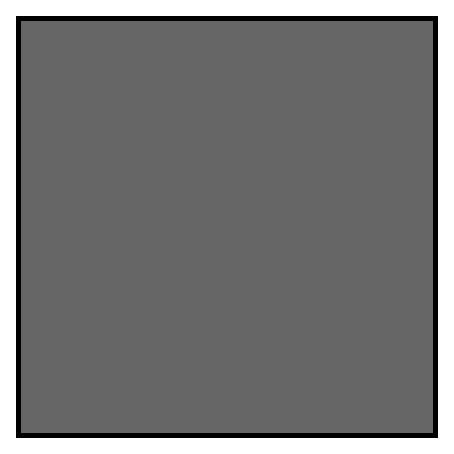
\includegraphics[width=0.75\textwidth]{example.eps}
% figure caption is below the figure
%\caption{Please write your figure caption here}
%\label{fig:2}       % Give a unique label
%\end{figure*}
%
% For tables use
%\begin{table}
% table caption is above the table
%\caption{Please write your table caption here}
%\label{tab:1}       % Give a unique label
% For LaTeX tables use
%\begin{tabular}{lll}
%\hline\noalign{\smallskip}
%first & second & third  \\
%\noalign{\smallskip}\hline\noalign{\smallskip}
%number & number & number \\
%number & number & number \\
%\noalign{\smallskip}\hline
%\end{tabular}
%\end{table}


%\begin{acknowledgements}
%If you'd like to thank anyone, place your comments here
%and remove the percent signs.
%\end{acknowledgements}

\begin{thebibliography}{}

\bibitem [\protect\citeauthoryear{Beer}{1990}]{Beer} 
Beer T.: The Australian National Bushfire model project. Math Comput. Model. 13(12), 49-56 (1990)

\bibitem [\protect\citeauthoryear{Del Moral}{2014}]{Del Moral} 
Del Moral P, Murraly L.M.: Sequential Monte Carlo with Highly Informative Observations. Math Comput. Model. 13(12), 49-56 (1990)

\bibitem [\protect\citeauthoryear{Malathy}{2011}]{Malathy} 
Malathy A., Baboo S.S.: An Enhanced Algorithm to Predict a Future Crime using Data Mining. Int. J. Comput. Appl. 21(1), 1-6 (2011)

\bibitem [\protect\citeauthoryear{Nakagawa}{2015}]{Nakagawa}
Nakagawa S.: Missing data. In: Fox G.A., Negrete-Yankelevich S., Sosa V.J. (eds.) Ecological Statistics: Contemporary theory and application, pp 81-105. Oxford University Press (2015). 

\bibitem[\protect\citeauthoryear{O'Neill}{2002}]{O'Neill}
O'Neill P.D., Roberts G.O.: Bayesian inference for partially observed stochastic epidemics. J. R. Stat. Soc. A. Stat. 162(1), 121-129 (2002)

\bibitem [\protect\citeauthoryear{Rubin}{1987}]{RubinMI}
Rubin D.B.: Multiple imputation for nonresponse in surveys. Wiley, New York (1987)

\bibitem [\protect\citeauthoryear{Rubin}{1987}]{Rubin}
Rubin D.B.: The Calculation of Posterior Distributions by Data Augmentation: Comment: A Noniterative Sampling/Importance Resampling Alternative to the Data Augmentation Algorithm for Creating a Few Imputations When Fractions of Missing Information Are Modest: The SIR Algorithm. J. Am. Stat. Assoc. 82(398), 543-546 (1987)

\bibitem [\protect\citeauthoryear{Tanner and Wong}{1987}]{Tanner}
Tanner M.A., Wong W.H.: The Calculation of Posterior Distributions by Data Augmentation. J. Am. Stat. Assoc. 82(398), 528-540 (1987)

\bibitem [\protect\citeauthoryear{Zhang}{2015}]{Zhang}
Zhang X-P. et al.: Multiple Imputations Particle Filters: Convergence and Performance Analyses for Nonlinear State Estimation with Missing Data. IEEE J. Sel. Top Signa. 9(8), 1536-1547 (2015)

\end{thebibliography}
\end{document}

